\documentclass[12pt]{article}
\usepackage[portuguese]{babel}
\usepackage{amsmath}
\usepackage{graphicx}
\newcommand{\numpy}{{\tt numpy}}   

\topmargin -.5in
\textheight 9in
\oddsidemargin -.25in
\evensidemargin -.25in
\textwidth 7in

\begin{document}
\medskip
\author{Tradução Juan Carlos Teran}
\title{TERMODINÂMICA}
\maketitle
O propósito deste capítulo é revisar alguns conceitos fundamentais da termodinâmica, que formam uma base essencial para o estudo da mecânica estatística. Os problemas 2.1-2.3 lidam com a primeira e a segunda leis e os conceitos associados de temperatura e potenciais termodinâmicos. Uma variedade de relações entre grandezas termodinâmicas, incluindo as relações de Maxwell, pode ser derivada desses princípios básicos, juntamente com as regras do cálculo diferencial, e os métodos para obter tais relações são ilustrados nos problemas 2.4 e 2.5. O problema 2.6 ilustra a natureza das mudanças de entropia em processos irreversíveis, enquanto os problemas 2.7-2.9 investigam as equações de estado de sistemas simples e suas consequências para vários processos termodinâmicos. Finalmente, o problema 2.10 lida com o tratamento termodinâmico de um material magnético e o problema 2.11 trata o comportamento de gases relativísticos em um cenário cosmológico.


 \begin{itemize}
     \item \textbf{Problema 2.1} Mostre que a energia livre de Helmholtz $F(T, V)$ de um sistema cujo volume é $V$ em contato com um banho térmico a temperatura $T$ é mínima no equilíbrio. Analogamente, mostre que a energia livre de Gibbs $G(T, P)$ de um sistema em contato com um banho a temperatura $T$ e pressão $P$ é mínima no equilíbrio.

     \textbf{Resposta:}
     Consideremos um sistema cujo volume $V$ é fixo e é colocado em contato com um banho térmico à temperatura $T$. Enquanto o sistema não estiver em equilíbrio com o banho, não podemos atribuir-lhe uma temperatura definida, portanto sua energia livre de Helmholtz $F$ não é uma função bem definida de temperatura e volume. Podemos, no entanto, tentar definir uma energia livre de não-equilíbrio por:
     \begin{equation*}
         F = U - TS
     \end{equation*}
     
     Aqui, entendemos por $U$ a energia interna do sistema, que está bem definida mesmo fora do equilíbrio, e por $T$ a temperatura do banho térmico (que também será a temperatura do sistema uma vez que o equilíbrio seja atingido). A entropia $S$ de não-equilíbrio do sistema não é simplesmente uma função de $U$ e $V$, mas depende dos detalhes do estado de não-equilíbrio. Podemos recorrer à declaração de Clausius da segunda lei para escrever a desigualdade:
     \begin{equation}
         \delta S \geq \frac{\delta Q}{T}
     \end{equation}
     onde $\delta Q$ é uma quantidade de calor transferida do banho térmico para o sistema. Como o volume do sistema é constante, nenhum trabalho é realizado enquanto esse calor é transferido, então a mudança na energia interna do sistema é $\delta U = \delta Q$. Como a temperatura $T$ do banho térmico é fixa, deduzimos que:
     \begin{equation}
         \delta F = \delta U - T \delta S = \delta Q - T \delta S \leq 0.
     \end{equation}
     Assim, $F$ sempre diminui à medida que o sistema se aproxima do equilíbrio e atinge um mínimo quando o equilíbrio é alcançado.
    
     Outra forma de abordar o problema é considerando a variação da energia livre de Helmholtz no equilíbrio, temos que
     \[
         \delta F = \delta U - \delta (S T)  
     \]
     \[
       \quad \quad \quad \quad = \delta U - S \delta T - T \delta S
     \]
    como a temperatura é constante $\delta T = 0$, assim
    \[
         \delta F = \delta U - T \delta S  
     \]
     da primeira lei da termodinâmica
     \begin{equation}
         \delta U = T \delta S - P \delta V
     \end{equation}

     como o volume é constante, temos que $\delta V = 0$, assim
     \[
     \delta U = T \delta S 
     \]
     pelo que 
     \[
     \delta F = T \delta S - T \delta S
     \]
     \[
      \delta F = 0
     \]
     Portanto, no equilíbrio térmico, a variação da energia livre de Helmholtz é zero, e  $F$ é estacionária. Agora, para verificar que  $F$ é mínima no equilíbrio, consideramos que o sistema tende a evoluir espontaneamente para estados que minimizem  $F$. Se $F$  diminui $\delta F < 0$ , ele se aproxima do equilíbrio. Assim, no equilíbrio:
     \[
     \delta F = 0 \quad \text{e} \quad F \, \text{é mínima}.
     \]

     No caso da energia livre de Gibbs $G = U + PV - TS$, devemos considerar um sistema cuja pressão P é mantida fixa, mas cujo volume pode variar à medida que se aproxima do equilíbrio. Nesse caso, as mudanças na energia são dadas por:
     \begin{equation}
         \delta U = \delta Q - P \delta V
     \end{equation}
     Um argumento semelhante ao apresentado acima resulta em:
     \begin{equation}
         \delta G = \delta U + P \delta V - T \delta S = \delta Q - T \delta S \leq 0
     \end{equation}
     Observe que $F$ é útil para descrever um sistema cuja temperatura e volume estão sujeitos a controle externo, enquanto $G$ é mais útil quando a temperatura e a pressão são controladas externamente.

     Outra forma de abordar a minimização da energia livre de Gibbs é considerando $G(T,P)$ como
     \[
     G = H - T S
     \]
    onde $H = U + P V$ é a entalpia.
    A variação da energia livre de Gibbs é
    \[
    \delta G = \delta H - \delta TS \quad \quad \vee \quad \quad \delta G =  \delta H - T \delta S - S \delta T
    \]
    
    como $T$ é constante $\delta T = 0$
    \begin{equation}
        \delta G = \delta H - T \delta S
    \end{equation}
    mas a variação da entalpia é 
    \[
    \delta H = \delta U + \delta PV \quad \quad \vee \quad \quad \delta H = \delta U + P \delta V + V \delta P
    \]
    como P é constante
    \begin{equation}
        \delta H = \delta U + P \delta V
    \end{equation}
    substituindo (3) em (7)
    \[
     \delta H = (T \delta S - P \delta V) + P \delta V
    \]
    \begin{equation}
       \delta H = T \delta S
    \end{equation}
    substituindo (8) em (6)
    \[
    \delta G = T \delta S - T \delta S = 0
    \]
    Portanto, no equilíbrio, a variação da energia livre de Gibbs é zero, e $G$ é estacionária. Analogamente ao caso da energia livre de Helmholtz, o sistema evolui espontaneamente para minimizar $G$. No equilíbrio:
    
    \[
    dG = 0 \quad \text{e} \quad G \, \text{é mínima}.
    \]
     \item \textbf{Problema 2.2} Discuta a possibilidade de um sistema físico ter uma temperatura negativa.
     \textbf{Resposta:} Para que um sistema físico tenha uma temperatura negativa, deve ocorrer uma inversão na relação usual entre energia e entropia. Ou seja, em vez de a entropia aumentar com a energia, ela diminui à medida que a energia interna aumenta. Isso implica que:
     \[
     \frac{\partial S}{\partial U} < 0
     \]
     Consequentemente, conforme a definição de temperatura:
     \[
     T < 0
     \]
     Esse comportamento é possível em sistemas físicos que possuem um limite superior para a energia, ou seja, sistemas nos quais a energia das partículas não pode ser aumentada indefinidamente. Em tais sistemas, a entropia atinge um máximo para uma certa energia, e, além desse ponto, se a energia aumentar mais, a entropia começa a diminuir, levando a uma temperatura negativa.
     
     Considere um sistema de energia limitada. Ou seja, o sistema tem uma energia mínima possível, que podemos considerar como sendo
     \[
     U = 0
     \]
     e uma energia máxima possível, digamos $U_{max}$. Nesse sistema, é provável que muito poucos microestados (talvez apenas um) correspondam a $U = 0$ e também que muito poucos correspondam a $U = U_{max}$. Assim, a entropia $S(U)$ é muito pequena tanto em $U = 0$ quanto em $U = U_{max}$, e há alguma energia intermediária $U*$ na qual $S(U)$ é máxima. A temperatura inversa 
     \[
     T^{-1} = \frac{\partial S}{\partial U}
     \]
     é zero.
     \begin{figure}
         \centering
         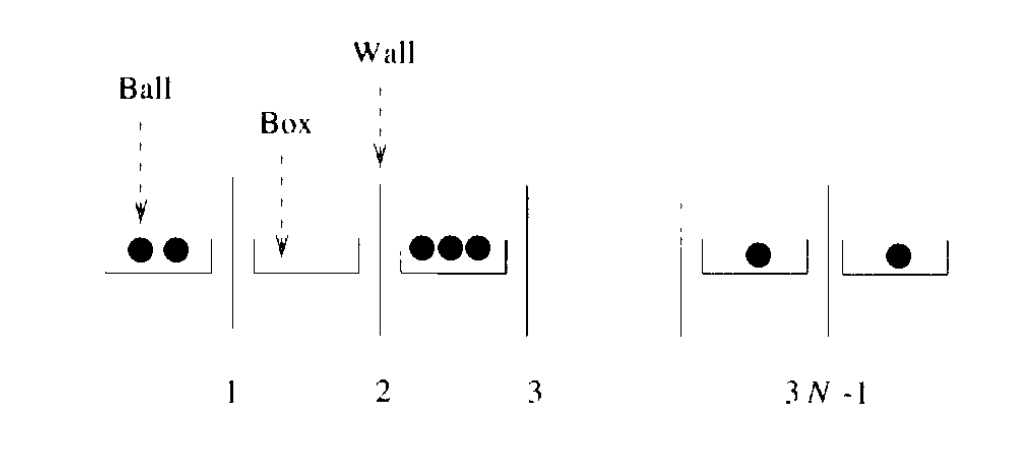
\includegraphics[width=0.5\linewidth]{image.png}
         \caption{Regiões de Temperatura Positiva e Negativa para um Sistema de Energia Limitada}
         \label{fig:enter-label}
     \end{figure}
Em $U = U^{*}$, a temperatura é positiva para $U < U^{*}$ e negativa para$ U > U^{*}$ (figura 1). Note que as temperaturas $T = +\infty$ e $T = -\infty $ correspondem ao mesmo estado, $T^{-1} = 0$. Além disso, um estado de temperatura negativa tem maior energia e, consequentemente, é mais quente que um estado de temperatura positiva. A declaração de Clausius sobre a segunda lei nos diz que o calor não flui espontaneamente de um corpo mais frio para um corpo mais quente, então o sistema não pode ser aquecido a uma temperatura infinita ou negativa por um influxo de calor, desde que seus arredores estejam a uma temperatura positiva finita. O calor sempre fluirá para fora de um sistema de temperatura negativa em contato com um sistema de temperatura positiva.

No entanto, é possível criar um estado de temperatura negativa por meios indiretos. O exemplo clássico é o de uma coleção de momentos magnéticos de núcleos atômicos, que interagem muito fracamente com os demais graus de liberdade em seu material hospedeiro e podem ser considerados efetivamente como um sistema isolado. A energia de um momento magnético (ou spin, para simplificar) é apenas aquela devido à sua orientação em um campo magnético aplicado. O sistema tem sua energia mínima quando todos os spins estão paralelos ao campo e sua energia máxima quando todos estão antiparalelos ao campo. O estado de temperatura infinita de entropia máxima corresponde a orientações completamente aleatórias dos spins. Em uma temperatura positiva baixa, os spins estarão predominantemente paralelos ao campo. Se a direção do campo for invertida rapidamente, os spins se encontrarão predominantemente antiparalelos ao campo e, portanto, em um estado de temperatura negativa.
     
     \item Problema 2.3 Compare a diminuição na entropia do cérebro de um leitor durante a leitura de um livro com o aumento na entropia devido à iluminação (por meio de uma lâmpada elétrica).
 \end{itemize}




\end{document}
